\chapter{Padrões Criacionais}

\section{Factory Method}

O padrão Factory Method tem como objetivo oferecer, através de uma 
classe Factory, uma interface para a criação de objetos. Esses objetos, 
porém, podem ser configurados através de classes que herdam de Factory.


\begin{figure}[htb]
	\caption{\label{fmethod_struct}Estrutura do Factory Method}
	\begin{center}
	    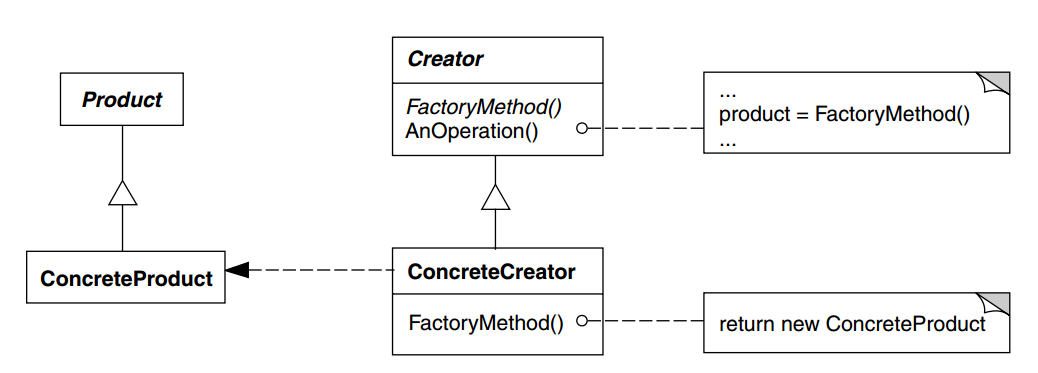
\includegraphics[scale=0.4]{5_padroes-contexto-funcional/5.1_criacionais/5.1.1_factory-method/diagram.png}
	\end{center}
\end{figure}

Exemplo Orientado a Objetos:

\begin{lstlisting}[caption={Factory Method Orientado a Objetos},label=oofactory]
    
    trait Product{
        def doStuff() : Unit
    }

    class ConcreteProduct extends Product(){

        def doStuff() : Unit = {
            
        }
    }

    abstract class Creator(){

        def someOperation() : Unit = {
            var p = createProduct()
            p.doStuff()
        }

        def createProduct() : Product
    }

    class ConcreteCreator() extends Creator{

        def createProduct() : Product = {
            return new ConcreteProduct()
        }
    }

\end{lstlisting}

Contexto Funcional:

\begin{lstlisting}[caption={Factory Method Funcional},label=fpfactory]
    
    

\end{lstlisting}